%! TEX rootmain.tex

\chapter{Lip-Driven Brass Instruments}

Lip-driven brass instruments can be viewed as coupled systems in which a self-oscillating lip valve interacts with an acoustic resonator shaped like a horn. The chapter surveys how the geometry of the bore affects resonances and playing behavior, and how mouthpieces contribute to both impedance matching and control. Radiation mechanisms are then discussed, together with practical tone-shaping devices such as slides, valves, and mutes. The treatment concludes by revisiting excitation and nonlinear effects in performance conditions and by outlining less conventional design choices that deviate from standard brass-instrument archetypes.

\section{Horn Profiles}

\begin{figure}[!htb]
\centering
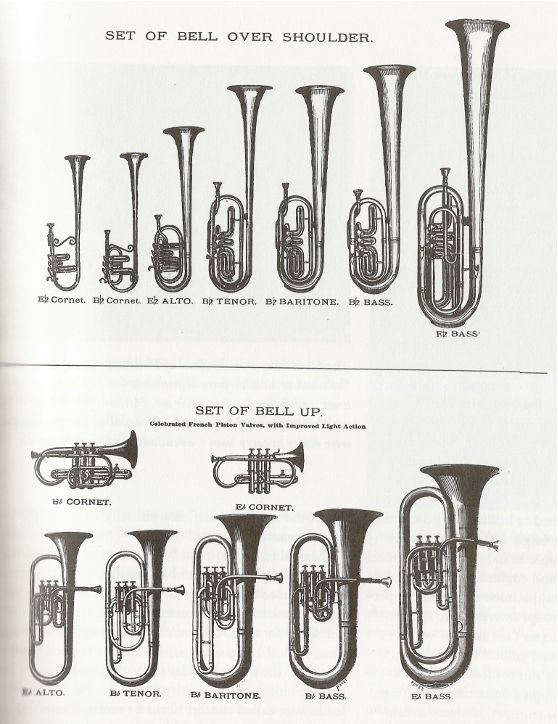
\includegraphics[width=0.5\linewidth]{00_Images/05_chapter/img34.jpg}
\caption{Overview of lip-driven brass instruments}
\label{fig:brass_overview}
\end{figure}

\subsection{Overall Geometrical Features}

Most brass instruments can be idealized as a cylindrical section connected to a flaring part. If the flaring portion is kept relatively short, for instance, not exceeding about one third of the total length, there remains enough geometrical flexibility to adjust the resonance frequencies of the modes through design choices in the profile. A reasonable approximation for many instruments, especially historical ones, is a cylindrical tube connected to a more-or-less conically expanding section of comparable length, terminated at the open end by a short region of more rapid flare. A representative overview of lip-driven brass instruments and their typical geometrical variety is shown in figure \ref{fig:brass_overview}.

\subsection{Conical Expansion And Tone}

Gently toned instruments typically exhibit a conical expansion over a large fraction of their length, up to about two thirds, with a small cone angle. In contrast, brightly toned trumpets and trombones tend to have a shorter expanding section and a more pronounced flare concentrated at the bell. For compound horns, the mode distribution is not described by a simple analytical sequence, although the series of input-impedance maxima remains more-or-less harmonic. 

\subsection{Bessel Horns}

A close approximation to the horn shape of a real brass instrument is provided by the Bessel horn model. If the mouth of the horn is located at \( x_0 \), the bore radius \( a \) as a function of the axial coordinate \( x \) is written as
\[
a = b(x - x_0)^{-\gamma}
\]
where \( \gamma \) controls the flare of the horn and \( b \) is a scaling constant. The effect of the flaring parameter on Bessel-horn profiles is illustrated in figure \ref{fig:bessel_profiles}.

\begin{figure}[!htb]
\centering
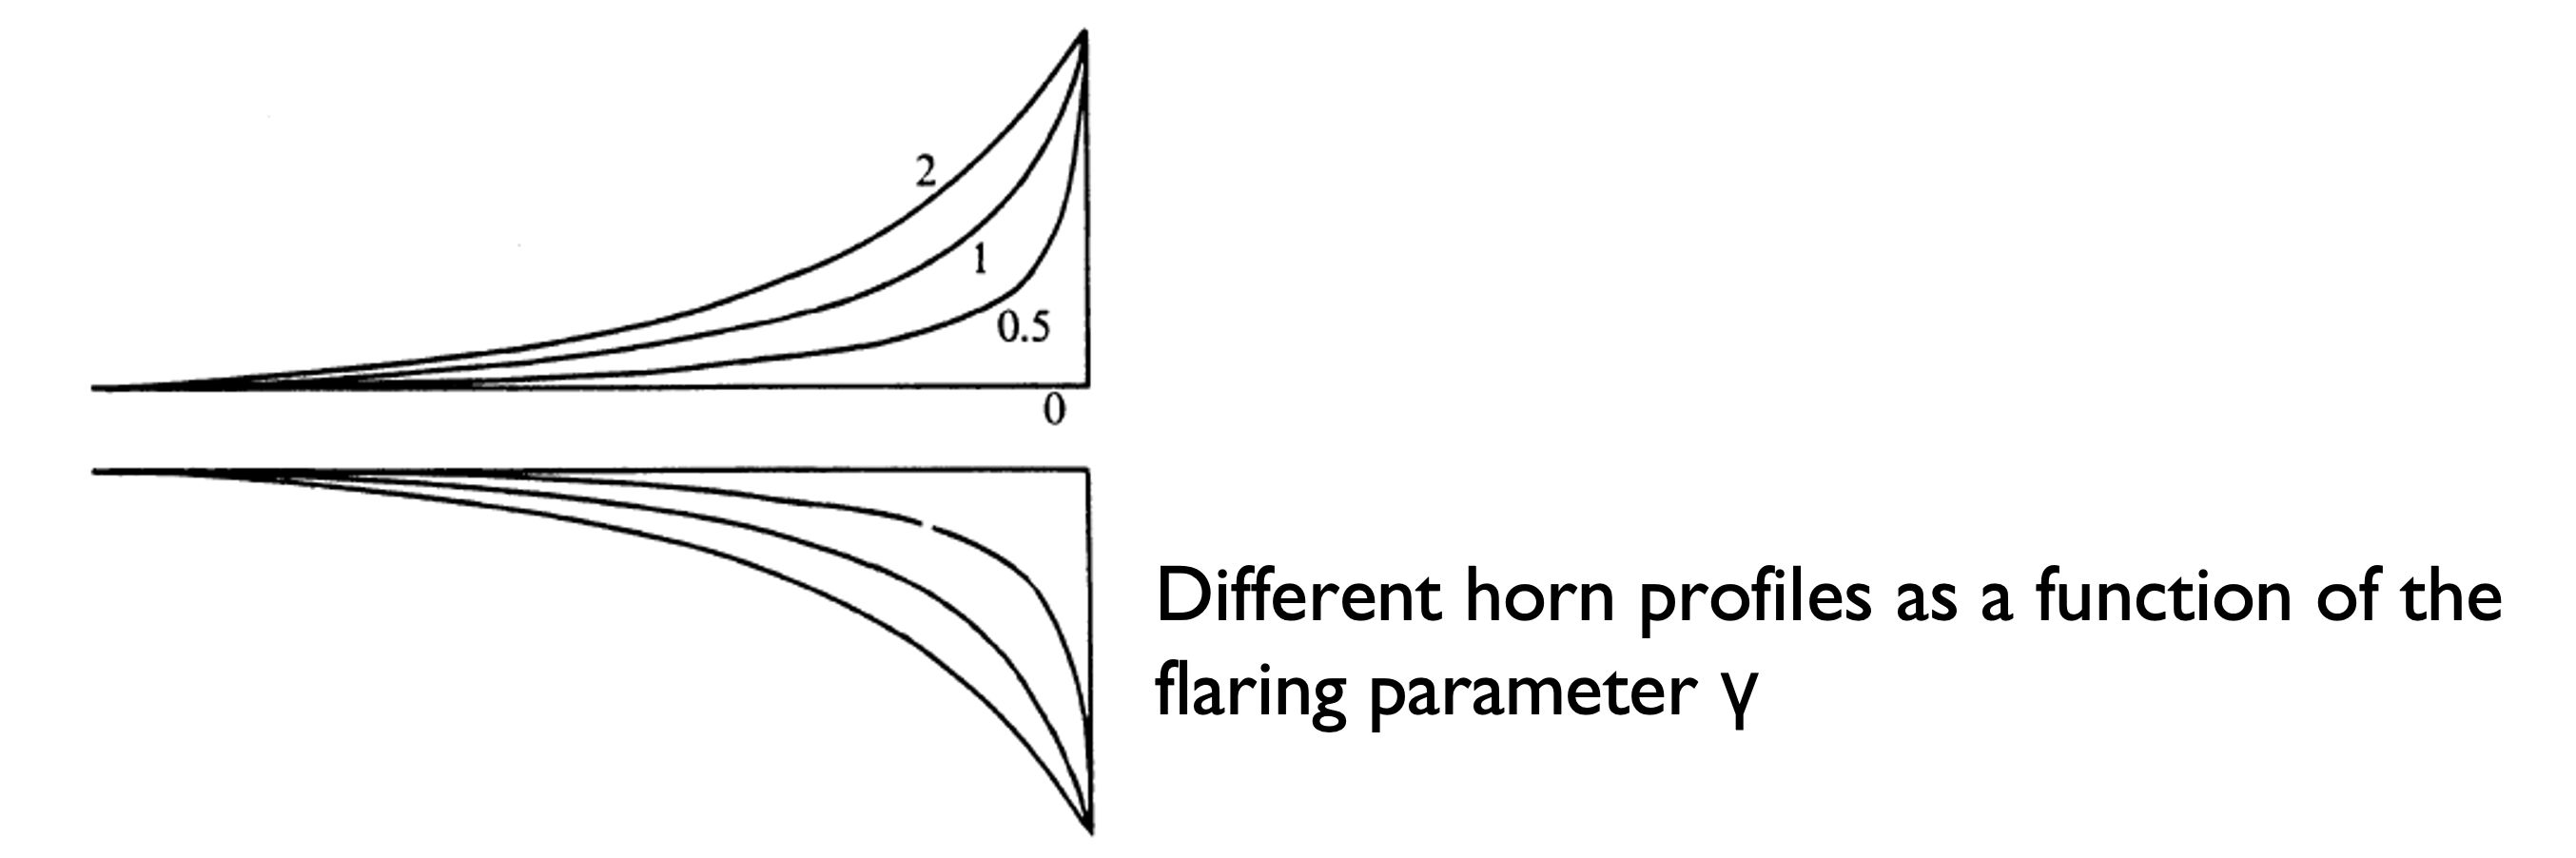
\includegraphics[width=0.7\linewidth]{00_Images/05_chapter/img79.jpg}
\caption{Bessel horn profiles for different values of the flare parameter}
\label{fig:bessel_profiles}
\end{figure}

\subsection{Impedance Maxima And Mode Series}

For a Bessel horn coupled to a tube of length \( l \), the frequencies of the impedance maxima can be approximated by
\[
f_n \approx \frac{c}{4(l + x_0)}
\left[(2n - 1) + \beta\sqrt{\gamma(\gamma + 1)}\right]
\]
where \( c \) is the sound speed and the coefficient \( \beta \) is about \( 0.6 \) for \( \gamma < 0.8 \) and about \( 0.7 \) for \( \gamma > 0.8 \). A few practical consequences follow from this description:

\begin{itemize}
    \item For \( \gamma = 1 \), the resonances are approximately harmonic, with
    \[
    f_n \approx \frac{nc}{2(l + x_0)}
    \]
    \item Instruments in the trumpet and trombone families typically correspond to \( \gamma \approx 0.7 \). Such horns can connect smoothly to cylindrical tubes, but their shape usually needs to be adjusted during design to obtain well-aligned reference resonances.
    \item The intended mode series is often tuned to approximate \( (0.7, 2, 3, 4, \dots)f_0 \). The first resonance is therefore strongly out of alignment, produces a very weak sound, and is not used in normal playing.
    \item Skilled players may nevertheless exploit nonlinear effects to produce a pedal note near \( f_0 \), relying on cooperation with the harmonically related higher resonances.
\end{itemize}

The relation between horn profile and the series of impedance maxima is illustrated in figure \ref{fig:impedance_maxima_series}.

\begin{figure}[!htb]
\centering
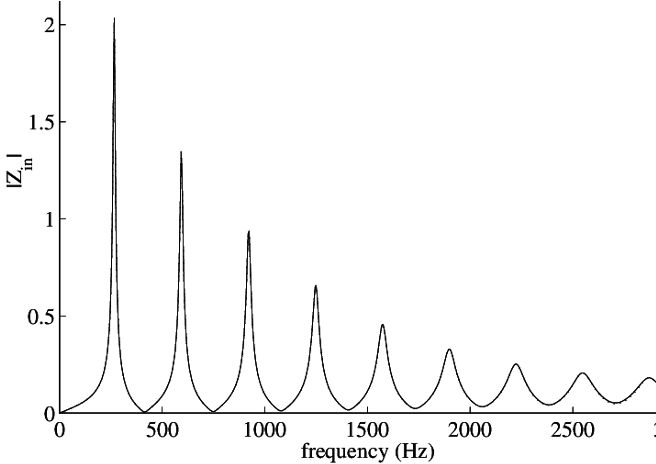
\includegraphics[width=0.7\linewidth]{00_Images/05_chapter/img93.jpg}
\caption{Impedance maxima and mode series in brass instruments}
\label{fig:impedance_maxima_series}
\end{figure}

\section{Mouthpieces}

The mouthpiece cup size roughly follows the size of the instrument as a whole. The player’s lips press against the smooth rim and cup surface, which provides comfortable mechanical support while allowing the lips to vibrate. The cup communicates with the instrument through a constricted passage (the throat), whose diameter is considerably smaller than the main bore. Mouthpieces also differ systematically across instrument families. Typical trumpet mouthpieces exhibit a relatively shallow cup and a narrow throat, while horn mouthpieces tend to have a deeper cup and a different internal contour, reflecting distinct requirements in impedance shaping and playing feel. 

\subsection{Lumped Model}

In acoustic terms, the detailed contour of the mouthpiece is less important than the cup volume and the diameter of the constricted passage. Representative mouthpiece profiles for different brass instruments are shown in figure \ref{fig:mouthpiece_profiles}.

\begin{figure}[!htb]
\centering
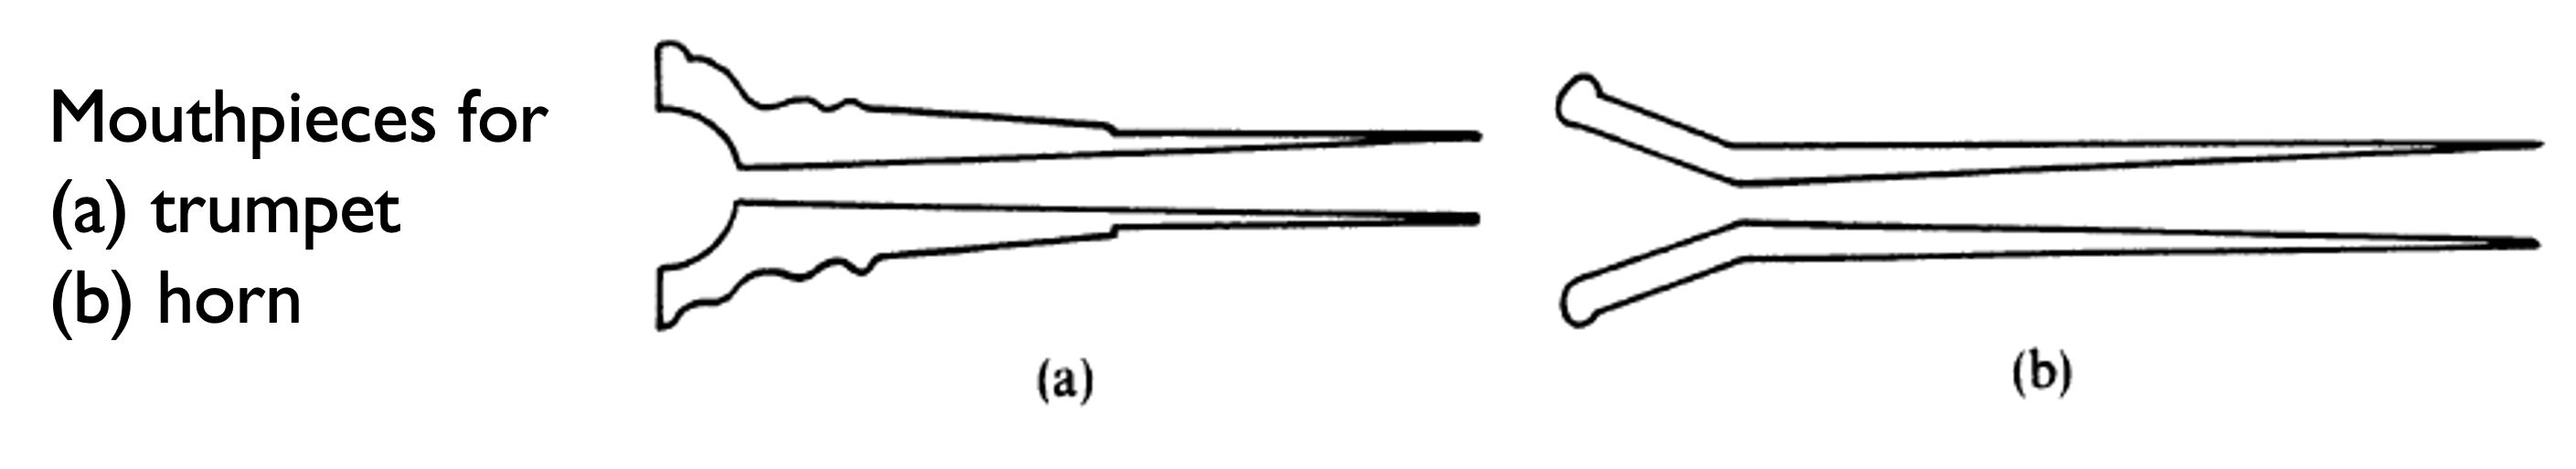
\includegraphics[width=0.7\linewidth]{00_Images/05_chapter/img103.jpg}
\caption{Mouthpiece profiles (e.g., trumpet versus horn)}
\label{fig:mouthpiece_profiles}
\end{figure}

The cup volume \( V \) acts as an acoustic compliance,
\[
C = \frac{V}{\rho c^{2}}
\]
where \( \rho \) is the air density and \( c \) is the speed of sound. The constriction behaves as a series of inertances,
\[
L = \frac{\rho l_c}{S_c}
\]
where \( S_c \) is the cross-sectional area of the constriction and \( l_c \) is its effective length. An additional dissipative element \( R \) in series with \( L \) represents viscous and thermal losses in the narrow passage.

\subsection{Coupling With The Resonator}

A convenient representation of the complete instrument is obtained through an electro acoustic analog: the cup compliance \( C \) loads the input, the constriction contributes the series elements \( L \) and \( R \), and the horn (or tube) contributes its own input impedance. A lumped (electro-acoustic) representation of the mouthpiece and its loading is shown in figure \ref{fig:mouthpiece_lumped_analog}.

\begin{figure}[!htb]
\centering
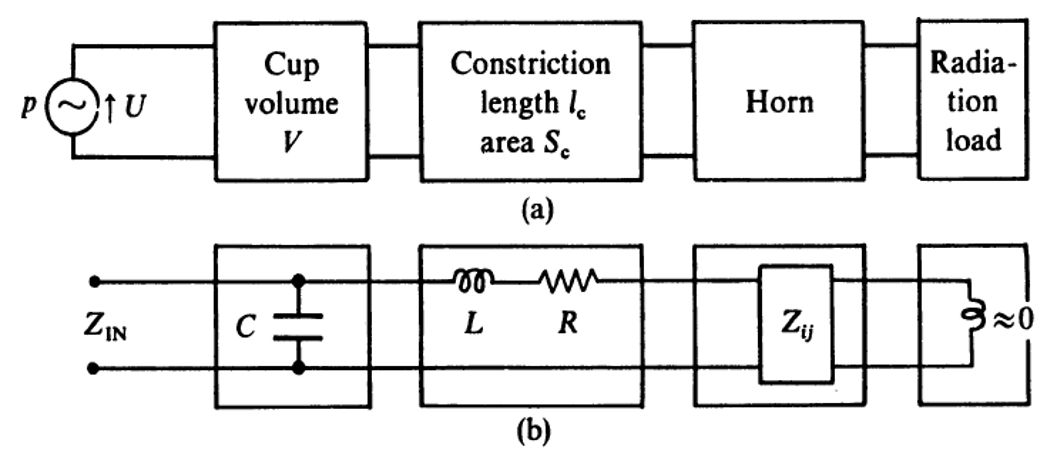
\includegraphics[width=0.7\linewidth]{00_Images/05_chapter/img117.jpg}
\caption{Lumped electro-acoustic analog of the mouthpiece and associated loads}
\label{fig:mouthpiece_lumped_analog}
\end{figure}

In this framework, the radiation impedance at the open end of the horn can be set to zero as a first approximation, since the dominant losses are attributed to wall losses along the horn. To make the coupling explicit, consider a mouthpiece connected to a simple cylindrical tube of length \( l \) and cross-sectional area \( S \). The input impedance of the tube is
\[
Z_{p} = jZ_{0}\tan(kl)
\qquad
Z_{0} = \frac{\rho c}{S}
\]
Wall losses are included by using a complex wavenumber
\[
k = \frac{\omega}{c} - j\alpha
\qquad
\alpha \approx 2\times 10^{-5}\left(\frac{\omega}{S}\right)^{1/2}
\]
with angular frequency \( \omega \). The input impedance presented to the player’s lips is then
\[
Z_{\mathrm{in}} =
\frac{R + Z_{p} + j\omega L}
{1 - \omega^{2}LC + j\omega C(R + Z_{p})}
\]
This expression highlights that the overall input impedance contains contributions associated with the tube and the mouthpiece itself. In particular, the mouthpiece behaves as a Helmholtz resonator, with a peak driving-point impedance near
\[
\omega_{0} = (LC)^{-1/2}
\]
while the peak height and half-width are controlled by the magnitude of the losses in the tube. 

\subsection{Considerations}

A few design consequences follow from the coupled model.

\begin{itemize}
    \item The lip generator is a pressure-controlled system that functions best when working with very high impedance. This motivates matching the mouthpiece to the instrument so that the mouthpiece resonance reinforces impedance peaks over the main playing range.
    \item The mouthpiece impedance also influences, to a smaller extent, the tuning of the horn resonances.
    \item The balance of resonance peak heights over the playing range is important because an easy transition between successive resonances is required for musical flexibility.
\end{itemize}

For a \( (+,-) \) lip valve, the imaginary part of the lip valve admittance is always negative. Therefore, for exact resonance and maximum acoustic pressure in the mouthpiece, the instrument must present a balancing positive acoustic admittance at the open face of the mouthpiece cup. More generally, for a multi-mode passive resonator, the imaginary part of the impedance rises through zero as the frequency passes through each impedance maximum. To satisfy the resonance condition, the operating frequency must lie slightly above the passive resonance frequency of the mode in question. The opposite conclusion applies for a valve in the \( (+,+) \) configuration. Typical impedance curves for the pipe alone, the mouthpiece alone, and the coupled system are shown in figure \ref{fig:impedance_coupling}.

\begin{figure}[!htb]
\centering
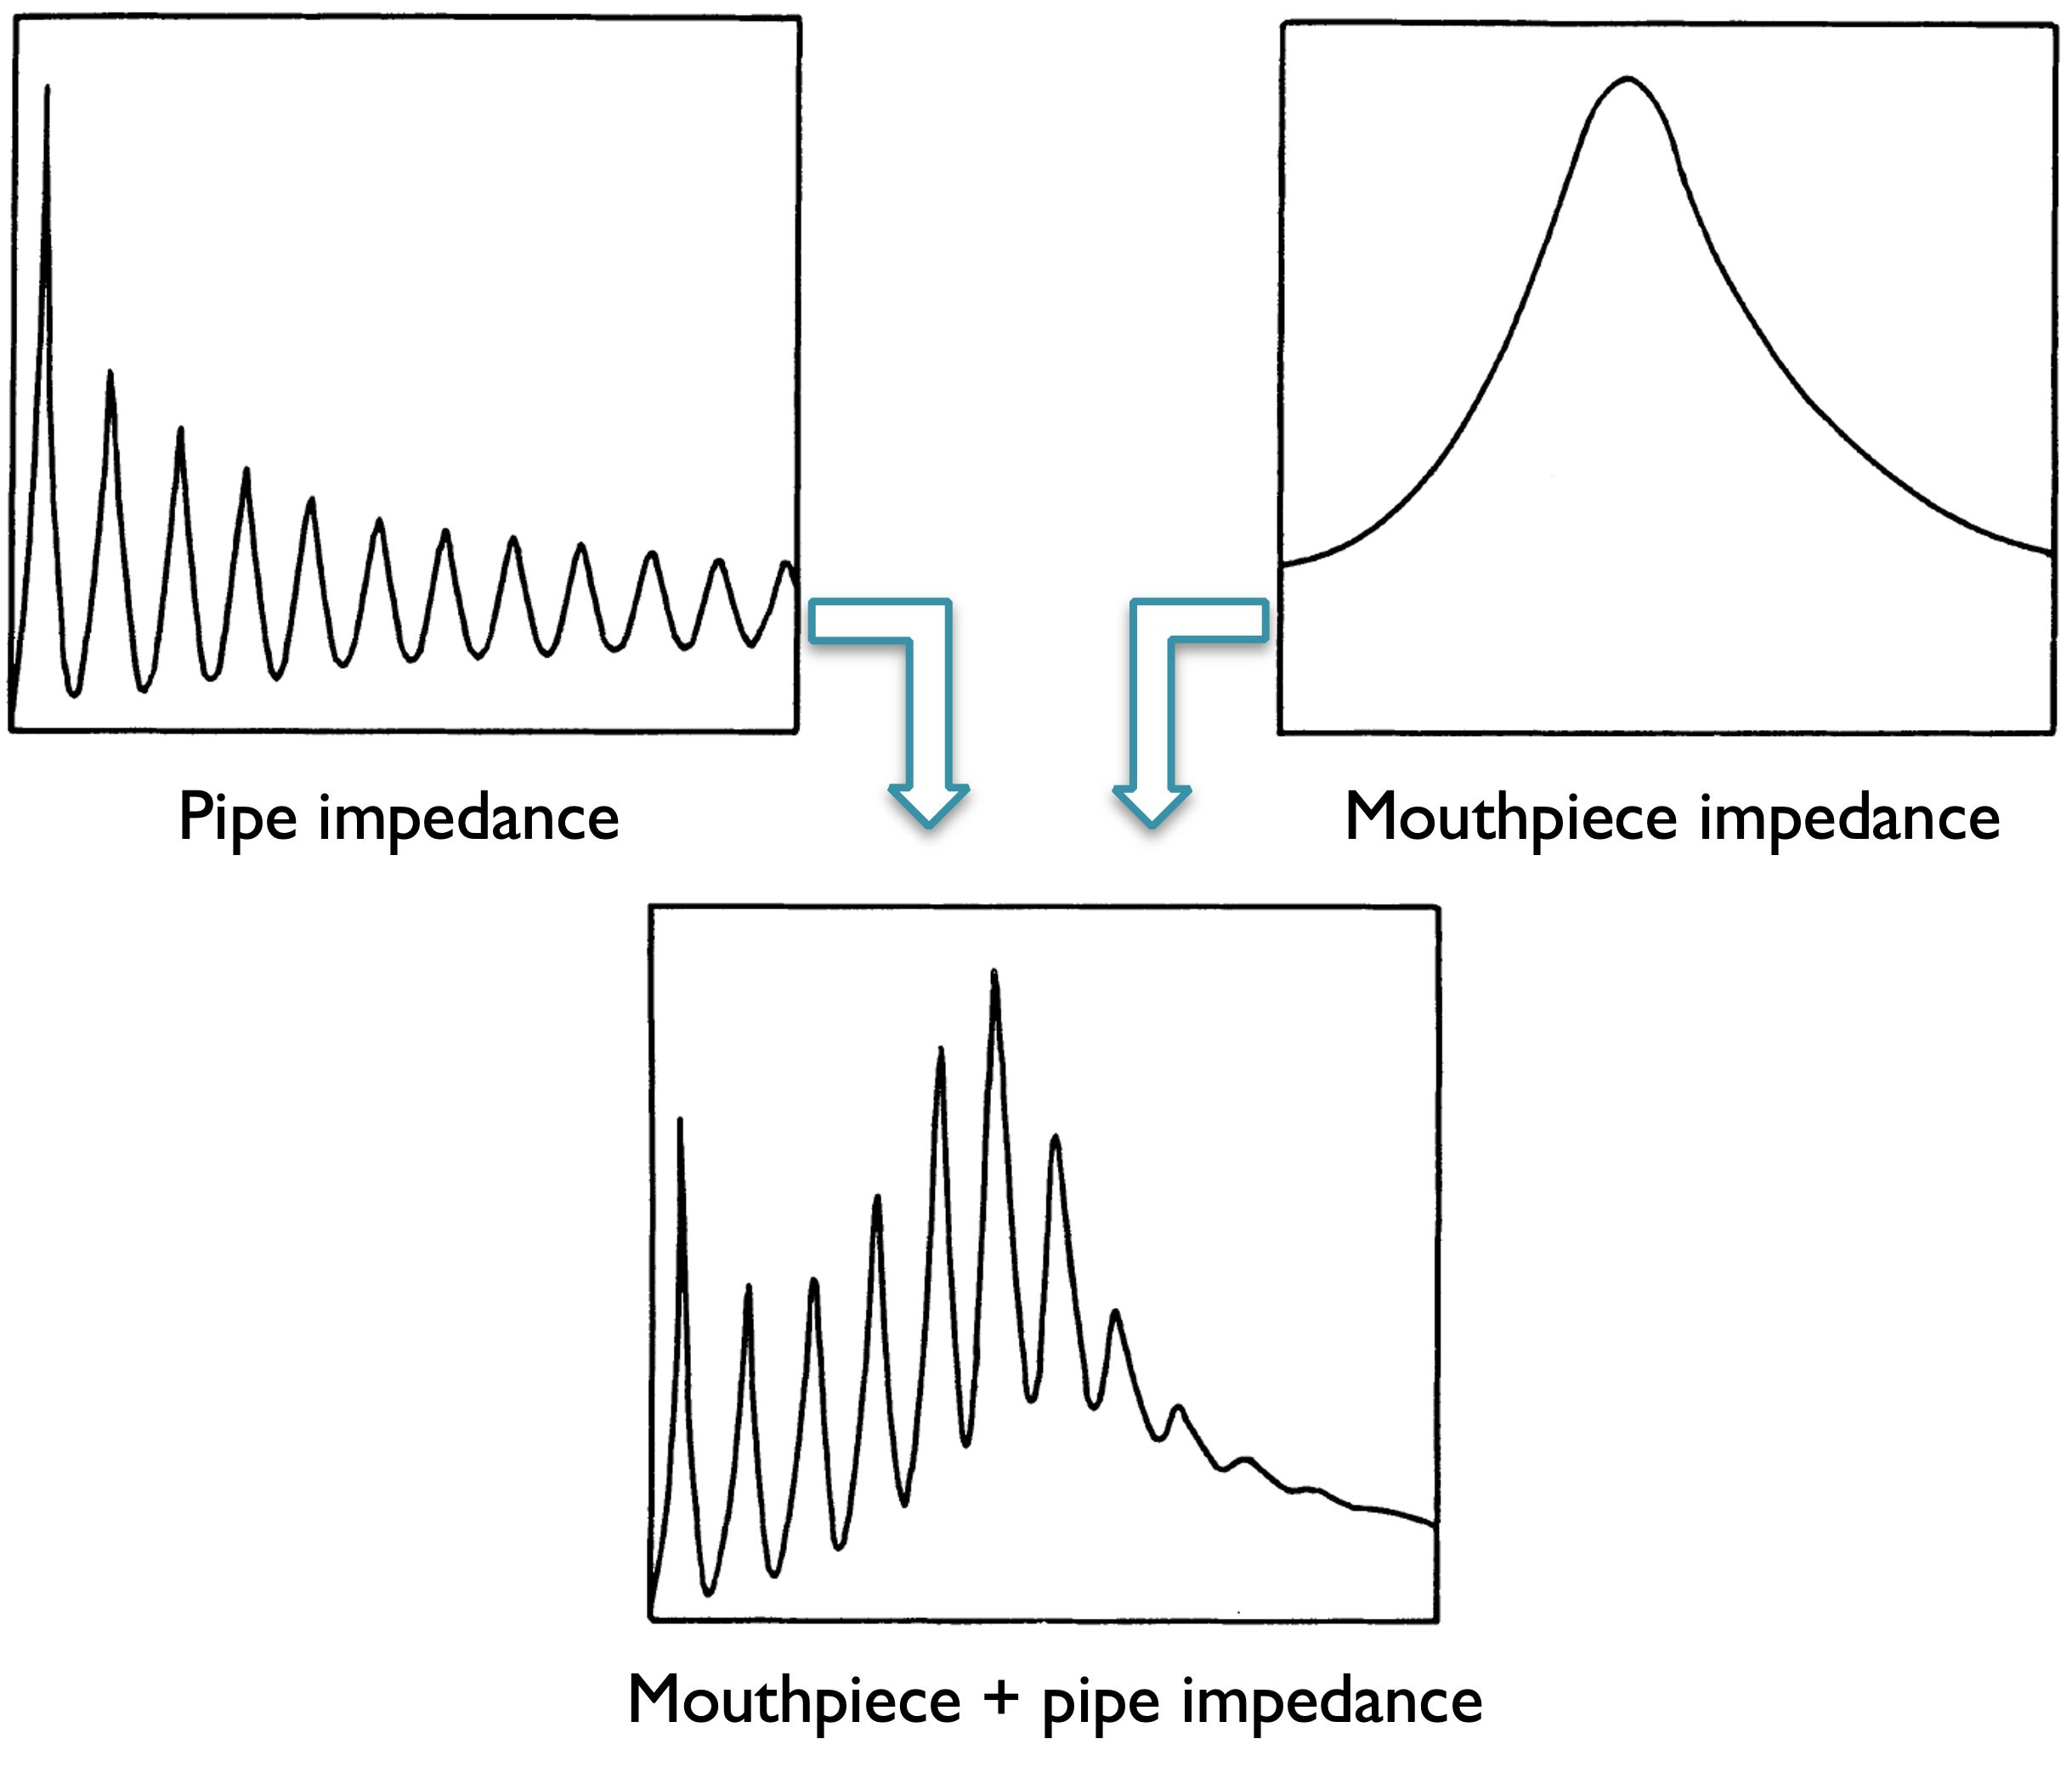
\includegraphics[width=0.7\linewidth]{00_Images/05_chapter/img125.jpg}
\caption{Impedance of pipe, mouthpiece, and coupled system}
\label{fig:impedance_coupling}
\end{figure}

\section{Radiation}

\subsection{Radiated Power}

At the horn mouth, radiation can be described through the radiation impedance \( Z_{\mathrm{rad}} \), whose resistive part \( R \) controls the radiated acoustic power. For a circular opening of radius \( a \), using \( k \) as the wavenumber and \( Z_{0} \) as the characteristic impedance associated with the mouth, the resistive term can be approximated as
\[
R \approx
\begin{cases}
Z_{0}\dfrac{(ka)^{2}}{4} & \text{for } ka \le 2 \\
Z_{0} & \text{for } ka \ge 2
\end{cases}
\]
If the acoustic particle velocity at the mouth is \( u \), the volume flow is
\[
U = \pi a^{2}u
\]
The total radiated power follows the corresponding asymptotic behaviors
\[
P \approx
\begin{cases}
\rho c\left(\pi a^{2}u^{2}\right)\dfrac{(ka)^{2}}{4} & \text{for } ka \le 2 \\
\rho c\left(\pi a^{2}u^{2}\right)(ka)^{2} & \text{for } ka \ge 2
\end{cases}
\]
These relations show that radiation efficiency increases with frequency in the low-frequency range. 

\subsection{Radiation Spectrum}

The radiation process can be viewed as a frequency-dependent transfer function: at low frequencies (relative to the cut-off), radiation is inefficient and the transfer magnitude increases with frequency, while above the cut-off it tends toward a flatter behavior. This trend is commonly summarized by plotting the transfer function versus frequency normalized to the cut-off frequency. A representative radiation spectrum (or radiation transfer) is shown in figure \ref{fig:radiation_spectrum_brass}.

\begin{figure}[!htb]
\centering
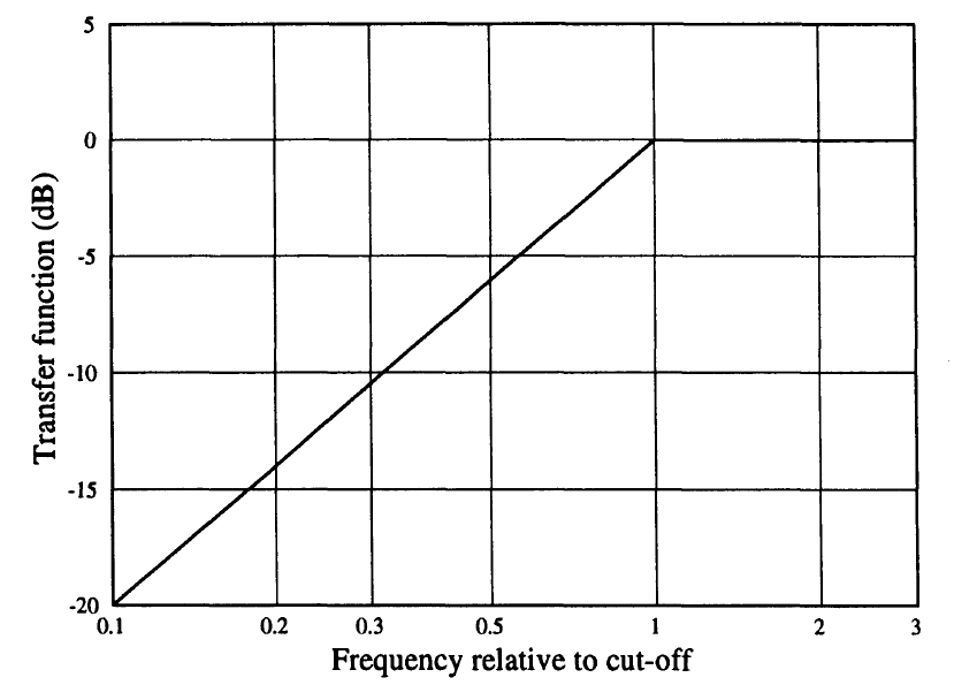
\includegraphics[width=0.7\linewidth]{00_Images/05_chapter/img133.jpg}
\caption{Radiation spectrum / transfer characteristics of a brass instrument}
\label{fig:radiation_spectrum_brass}
\end{figure} 

\subsection{Angular Dependency}

A useful directivity model is that of a baffled piston. The radiation intensity at angle \( \theta \) can be written as 
\[
\left[\frac{2J_{1}(ka\sin\theta)}{ka\sin\theta}\right]^{2}
\]
where \( J_{1} \) is the Bessel function of the first kind of order one. At low frequencies, the angular distribution is almost independent of \( \theta \). As frequency increases, radiation becomes progressively concentrated in the forward direction, and an intensity null appears at
\[
\theta_{0} = \sin^{-1}\left(\frac{3.8}{ka}\right)
\]
A practical rule is that frequencies above roughly \( 200/a \) are strongly concentrated along the horn axis. 

\section{Slides and Valves}

Slides and valves are used to fill the gaps between the lower resonances in order to produce a complete range of notes in the lower compass. 

\begin{itemize}
    \item Natural horns and Baroque trumpets did not include slides or valves. Apart from an extension shank or crook inserted between the mouthpiece and the instrument, the overall pitch could only be shifted to play in a different key. 
    \item A complete scale was therefore available only in the upper register, where adjacent resonances become sufficiently close.
    \item Additional mechanisms were needed to overcome this limitation and access intermediate notes in the lower range.
\end{itemize}

\subsection{Slides}

Ignoring the pedal note, the largest gap to be filled is between the second and third modes, which form a musical fifth and leave six notes in between. Since the frequency ratio of these modes is \( 2:3 \), covering the gap requires changing the effective tube length by about \( 50\% \),
\[
L' \approx \frac{3}{2}L
\]
because resonance frequencies scale approximately as \( f \propto 1/L \). A concrete example is provided by the tenor trombone. When the slide is closed, the bore length is approximately \SI{270}{\centi\meter} and
\[
f_2 \approx \SI{127}{\hertz}
\]
When the slide is fully open, the length increases to about \SI{405}{\centi\meter}, leading to
\[
f_2 \approx \SI{84}{\hertz}
\qquad
f_3 \approx \SI{127}{\hertz}
\]
so that the frequency region between \( f_2 \) and \( f_3 \) can be covered continuously by moving the slide. The main drawback is the large physical movement required between notes, which restricts execution speed and makes a true legato, without an audible gliding tone, nearly impossible. A typical tuning-slide arrangement is shown in figure \ref{fig:tuning_slide}.

\begin{figure}[!htb]
\centering
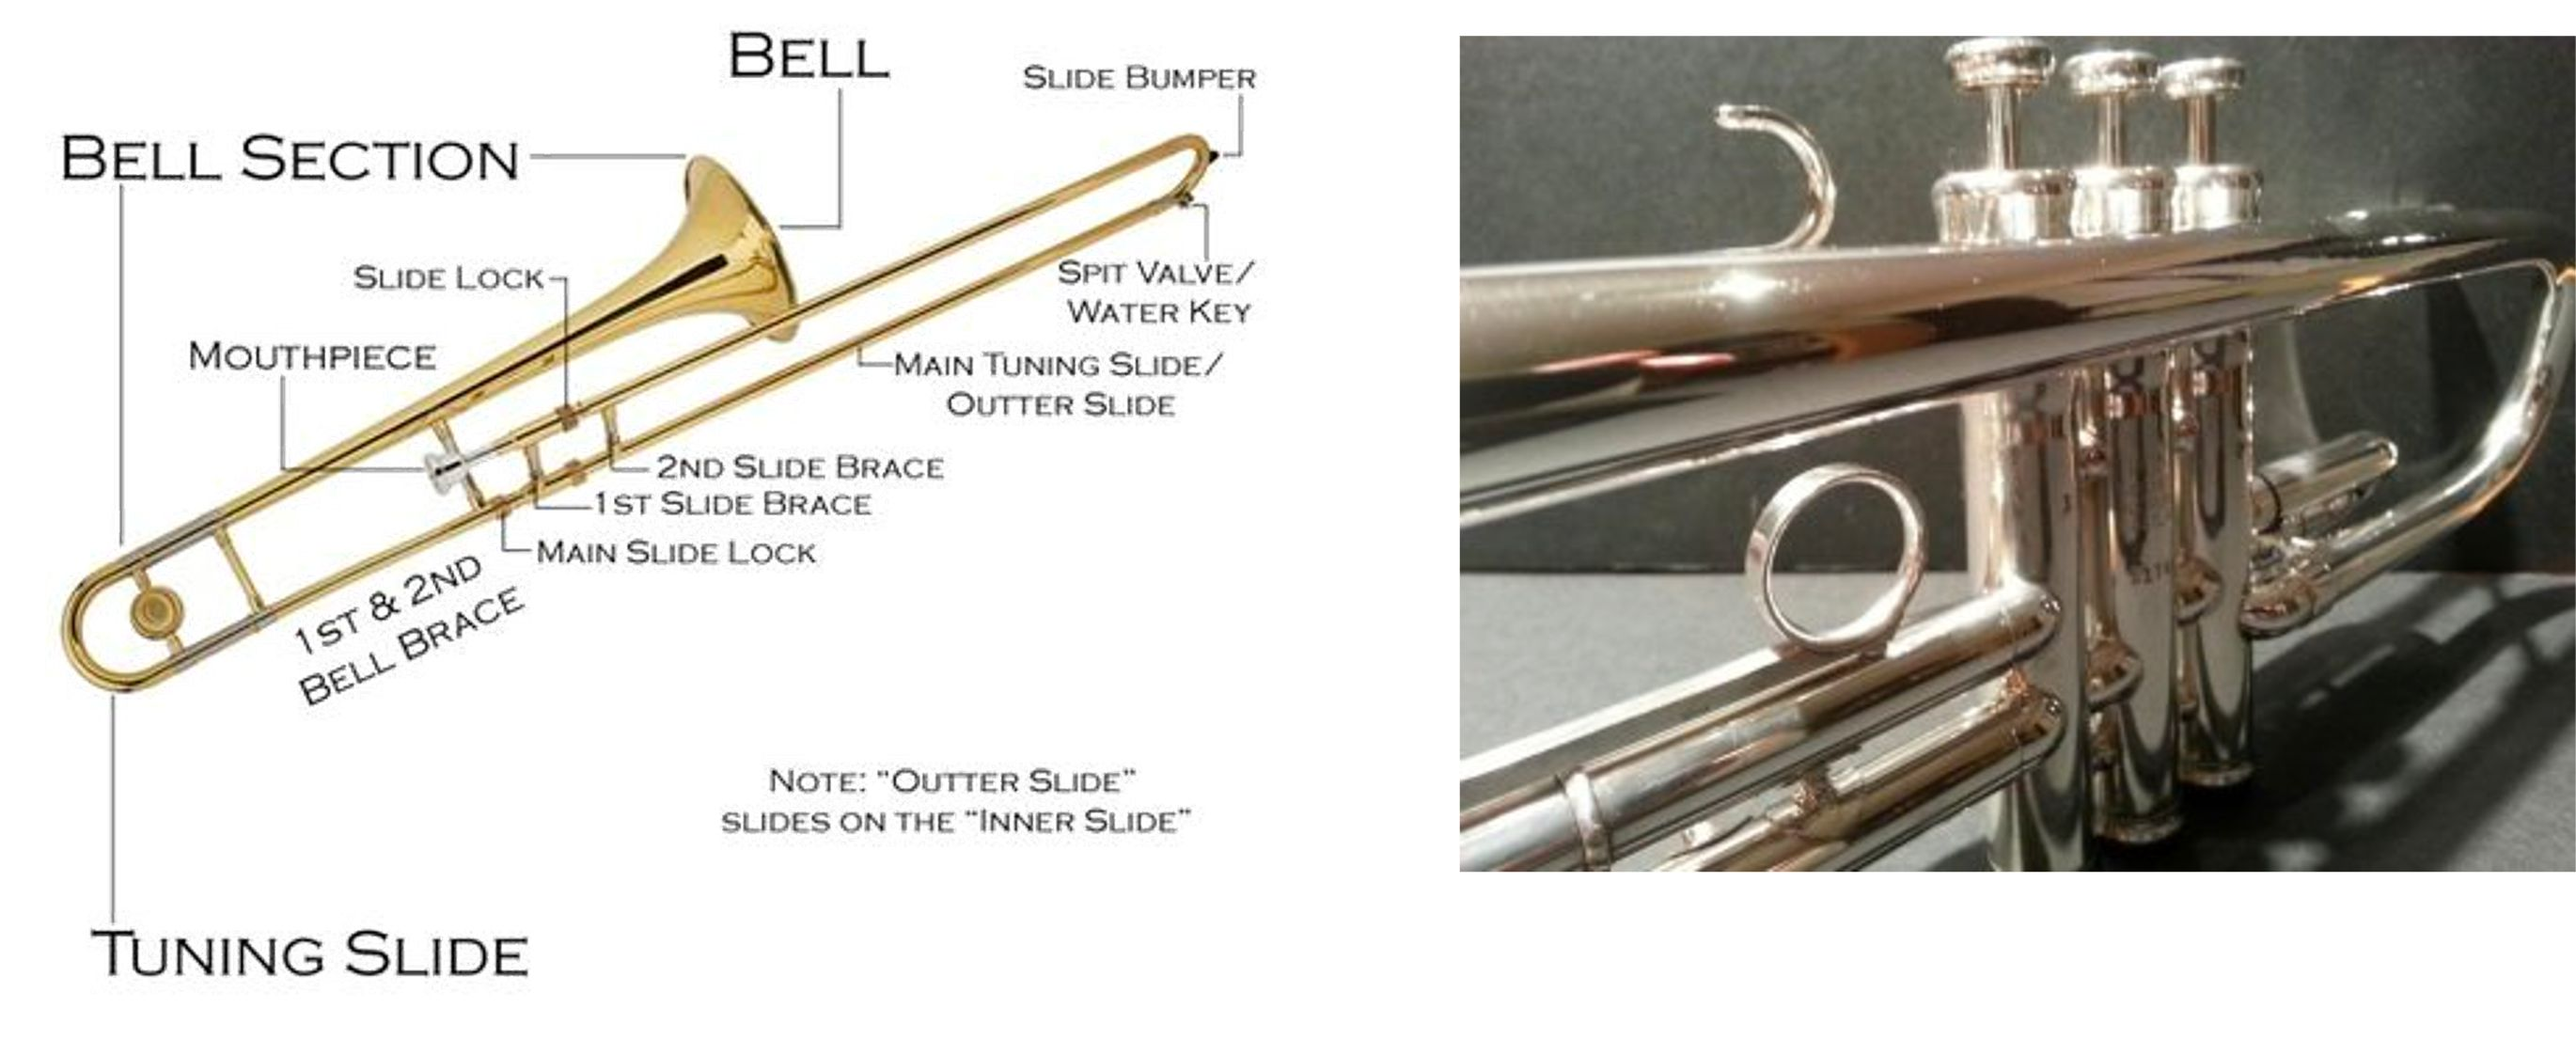
\includegraphics[width=0.7\linewidth]{00_Images/05_chapter/img141.jpg}
\caption{Tuning slide arrangement in brass instruments}
\label{fig:tuning_slide}
\end{figure}

\subsection{Valves}

The most widely adopted alternative to slides uses finger-operated valves to insert extra lengths of tubing into the cylindrical part of the instrument. Since each valve provides only two positions, at least three valves are needed, used in combination, to supply the six intermediate notes required to fill the large gap between modes 2 and 3. The operating principle and common valve configurations are illustrated in figure \ref{fig:valves_principle}.

\begin{figure}[!htb]
\centering
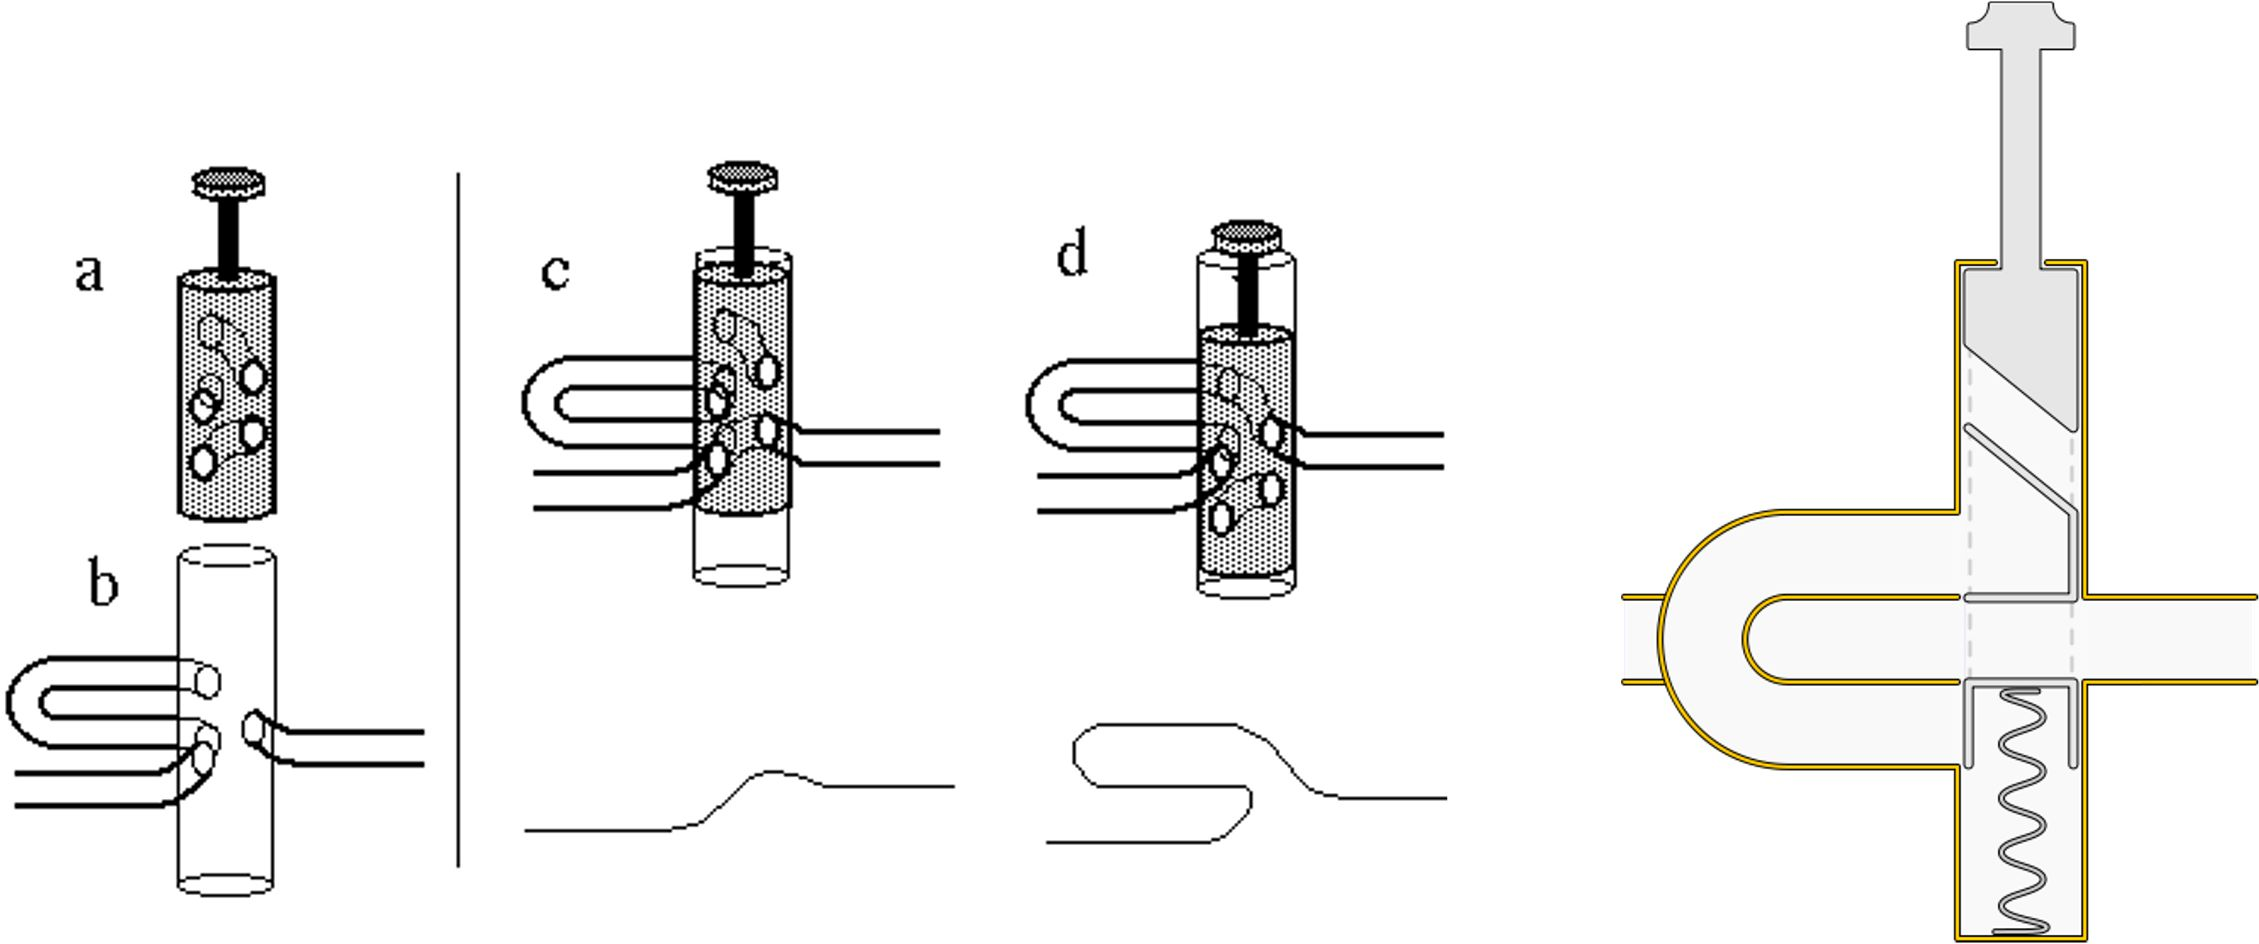
\includegraphics[width=0.7\linewidth]{00_Images/05_chapter/img151.jpg}
\caption{Valve principle and typical configurations}
\label{fig:valves_principle}
\end{figure}

\subsection{Valve Length Increments and Practical Tuning}

An equal-tempered semitone corresponds to a frequency change of about \( 6\% \). Therefore, to lower the frequency of a note by one semitone, the tube length must be increased by roughly a factor \( 1.06 \). If the required length extension for one semitone is written as \( 1 + x \), then a shift of \( n \) semitones requires
\[
(1 + x)^{n}
\]
which is larger than the linear increase \( 1 + nx \) obtained by combining \( n \) identical valves. This creates a tuning compromise for the usual \( 1 \), \( 2 \), and \( 3 \) semitone valves. 

\begin{itemize}
    \item If the three valves are tuned so that the total length equals \( (1 + x)^{n} \) when combined, then the individual semitone shifts become too sharp.
    \item If the valves are tuned so that each one individually produces exactly \( 1 \), \( 2 \), and \( 3 \) semitones, respectively, then pressing all three produces a total tube length that is too long, making the combined shift flat.
    \item A practical compromise is used: for instance, valve 3 may be tuned flat and valves \( 1+2 \) are used for the 3-semitone shift, while valve 3 is reserved for 4, 5, and 6 semitone shifts when combined with valve 1, valve 2, or both. 
\end{itemize}

Practical length increments required for pitch changes are summarized in figure \ref{fig:slide_extension_semitones}.

\begin{figure}[!htb]
\centering
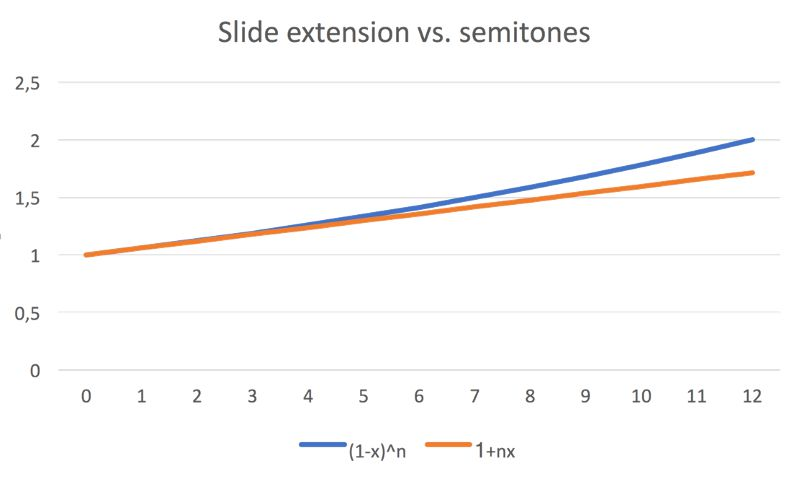
\includegraphics[width=0.7\linewidth]{00_Images/05_chapter/img157.jpg}
\caption{Slide extension (or added length) versus pitch change in semitones}
\label{fig:slide_extension_semitones}
\end{figure}

\section{Excitation and Nonlinearities}

\subsection{Small Amplitude Nonlinearities}

The small-amplitude description applies to gently blown notes. As discussed for reed- and lip-driven generators, the relation between acoustic volume flow and pressure is nonlinear. A convenient representation is a power-series expansion
\[
U = a_{1}p + a_{2}p^{2} + a_{3}p^{3}
\]
where the coefficients \( a_{n} \) are frequency dependent and may also encode a phase shift. Since the pressure is periodic, it can be written as a Fourier series
\[
p = \sum_{n} p_{n}\cos(n\omega t + \phi_{n})
\]
Consider a single flow component \( U \). The \( m \)-th order term in the nonlinear flow relation generates products of harmonics, leading to contributions of the form
\[
p_{i}p_{j}\cdots p_{k}\cos\left[(i \pm j \pm \cdots \pm k)\omega t + (\phi_{i} \pm \phi_{j} \pm \cdots \pm \phi_{k})\right]
\]
Collecting all terms at frequency \( n\omega \), one obtains an expression of the form
\[
U_{n}
= a_{n1}p_{n}
+ \sum_{k} a_{n2}p_{n\pm k}p_{k}
+ \sum_{j,k} a_{n3}p_{n\pm j\pm k}p_{j}p_{k}
+ \cdots
\]
showing explicitly how nonlinearities couple harmonic components. The lip generator is coupled to an instrument with input impedance \( Z(\omega) \). At the throat, the harmonic components satisfy
\[
p_{n} = Z_{n}U_{n}
\]
If only the fundamental is retained and terms above the third order are neglected, the governing relation can be reduced to:
\[
Z_{1}^{-1}p_{1} = a_{11}p_{1} + a_{13}p_{1}^{3}
\]
which yields the amplitude estimate
\[
p_{1} \approx \left[\frac{a_{11} - Z_{1}^{-1}}{-a_{13}}\right]^{1/2}
\]
With \( a_{11} > 0 \), \( a_{13} < 0 \), and \( \Re(Z_{1}) > 0 \), the fundamental pressure reaches its maximum when the instrument input impedance is maximal. The same conclusion applies to the first harmonic, whose pressure is maximized near an impedance maximum at \( 2\omega \).

\subsection{Large Amplitude Nonlinearity}

As the oscillation amplitude increases with blowing pressure, solving the coupled equations for pressure and flow becomes progressively more difficult, and determining the coefficients \( a_{nj} \) in the series description is no longer practical. At the same time, interactions among harmonics and harmonically driven pipe modes become stronger as higher harmonics grow. A more physical viewpoint is therefore required.  Representative large-amplitude waveforms of pressure and volume flow are shown in figure \ref{fig:brass_waveforms_pressure_flow}.

\begin{figure}[!htb]
\centering
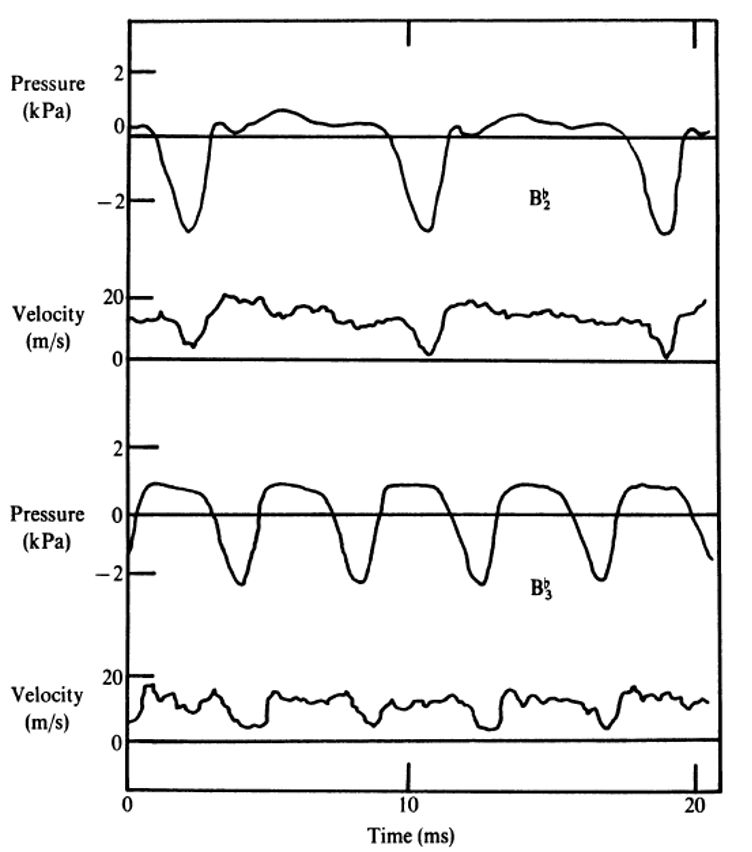
\includegraphics[width=0.7\linewidth]{00_Images/05_chapter/img165.jpg}
\caption{Large-amplitude pressure and volume-flow waveforms in a brass instrument}
\label{fig:brass_waveforms_pressure_flow}
\end{figure}

\paragraph{Pressure and Flow Waveforms}

Measurements of mouth-cup pressure and flow velocity for played trombone notes illustrate that, at high excitation, both waveforms can become strongly non-sinusoidal and noticeably asymmetric over the cycle. A simplified nonlinear relation between volume flow and mouthpiece pressure can be written as
\[
U = \gamma x(p_{0} - p)^{1/2}
\]
where \( x \) is the lip opening and \( \gamma \) is a constant. If the instrument is played at a resonance, it can be approximated by a simple acoustic resistance \( R \), so that \( p \approx UR \). Combining the two relations yields
\[
U \approx \frac{R\gamma^{2}x^{2}}{2}
\left[\left(1 + \frac{4p_{0}}{R^{2}\gamma^{2}x^{2}}\right)^{1/2} - 1\right]
\]

\paragraph{Approximations} Two limiting cases are useful:

\begin{itemize}
    \item If the lip opening is small and the blowing pressure is large, so that \( 4p_{0} \gg R^{2}\gamma^{2}x^{2} \), then
    \[
    U \approx \gamma x p_{0}^{1/2}
    \]
    \item If the lip opening is large and the blowing pressure is moderate, so that \( 4p_{0} \ll R^{2}\gamma^{2}x^{2} \), a second-order expansion gives
    \[
    U \approx \frac{p_{0}}{R} - \frac{p_{0}^{2}}{R^{3}\gamma^{2}x^{2}}
    \]
\end{itemize}

\paragraph{Time Dependent Behavior} Assume the effective lip opening follows an approximately sinusoidal motion,
\[
\gamma x \approx a_{0} + a\sin(\omega t)
\]
In the small-excitation limit,
\[
U \approx a_{0}p_{0}^{1/2} + ap_{0}^{1/2}\sin(\omega t)
\]
and the mouthpiece pressure is approximately \( R \) times this quantity. In the large-excitation case,
\[
U \approx \frac{p_{0}}{R} - \frac{p_{0}^{2}}{R^{3}(a_{0} + a\sin(\omega t))^{2}}
\]
If the lips close just once per cycle, one has \( a \approx a_{0} \), and the second term introduces a strongly distorted component. When \( \sin(\omega t) > 0 \), the correction is small and \( U \) saturates toward \( p_{0}/R \). When \( \sin(\omega t) = -1 \), the correction becomes large and negative and \( U \) drops well below zero. 

\paragraph{Final Considerations} In this simplified picture, the acoustic volume flow oscillates between extremes
\[
\frac{p_{0}}{R}
\qquad
-\frac{p_{0}^{2}}{R^{3}}
\]
leading to asymmetrical flow and pressure waveforms with a negative offset. Once the mouth cup flow waveform is known, it can be used as an input to the instrument impedance in order to determine the acoustic pressure in the mouth cup. At very high playing levels, further effects become relevant. The sound pressure level in the mouthpiece can reach about \SI{175}{\decibel}. At such levels, the wave equation becomes nonlinear, and in long bores, such as trumpets and trombones, shock waves can be produced.

\section{Spectral Features and Mutes}

\subsection{Spectral Features}

Both steady-state and transient properties of brass-instrument spectra can be summarized through a small set of robust trends.

\begin{itemize}
    \item The attack transient typically lasts \( 50 \pm \SI{20}{\milli\second} \), and this duration is approximately independent of the played note and the instrument. 
    \item The steady-state spectral envelope is characterized by a cutoff frequency: below the cutoff, radiated spectral components are roughly equal in amplitude or rise gradually with frequency, while above the cutoff, the amplitude decreases sharply as the frequency increases. 
    \item Typical slopes are in the range \SIrange{2}{4}{\decibel} per octave below the cutoff and \SIrange{15}{25}{\decibel} per octave above the cutoff.
    \item Playing more loudly shifts a larger fraction of radiated power into partials near and above the cutoff. Correspondingly, the slope below the cutoff increases and the slope above the cutoff decreases as intensity increases. 
    \item The cutoff frequency occurs in a comparable part of the frequency range for different instruments, so that spectral envelopes can be scaled and meaningfully superimposed. 
\end{itemize}

The comparison plot illustrates this scaling idea by showing that the mid-frequency envelopes of the trumpet, trombone, and tuba can be brought into close correspondence once the frequency axis is normalized appropriately, while retaining instrument-dependent deviations in level. 

\subsection{Mutes}

Mutes are especially effective in brass instruments because the radiation is dominated by the horn mouth, so the radiated sound can be altered in a controlled and repeatable way. A mute reduces the sound level, but the reduction is generally frequency dependent, so timbre is also modified. Different mute designs exploit this frequency dependence to produce characteristic tone colors. Two broad fitting strategies are commonly distinguished. Open mutes fit tightly in the instrument bell, while closed mutes are supported on cork pads, leaving an annular opening. Common mute types and their basic designs are summarized in figure \ref{fig:mute_types}.

\begin{figure}[!htb]
\centering
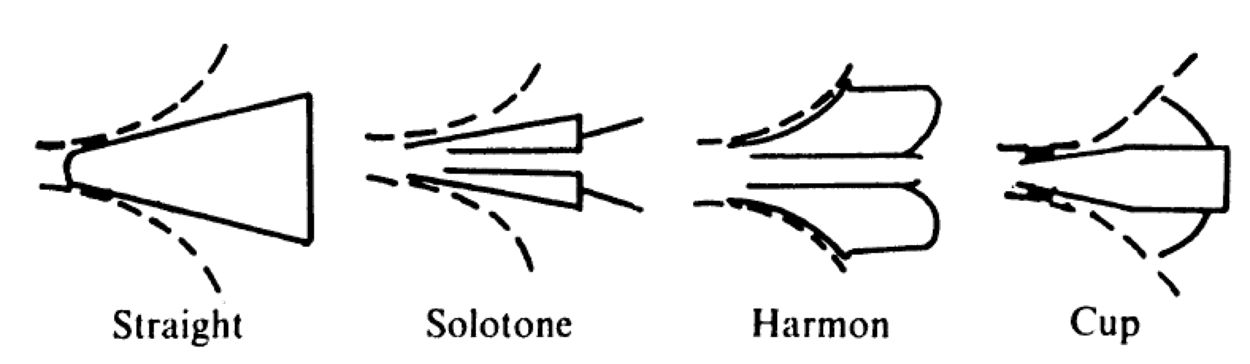
\includegraphics[width=0.7\linewidth]{00_Images/05_chapter/img183.jpg}
\caption{Examples of common brass mutes}
\label{fig:mute_types}
\end{figure}

\paragraph{Spectral Features} The spectrum plot compares the spectral envelopes of a normal B\( ^{\flat} \) cornet note with the same note played using various mutes. The curves show that different designs reshape the envelope in distinct ways across frequency, producing perceptually different brightness and coloration.

\begin{figure}[!htb]
\centering
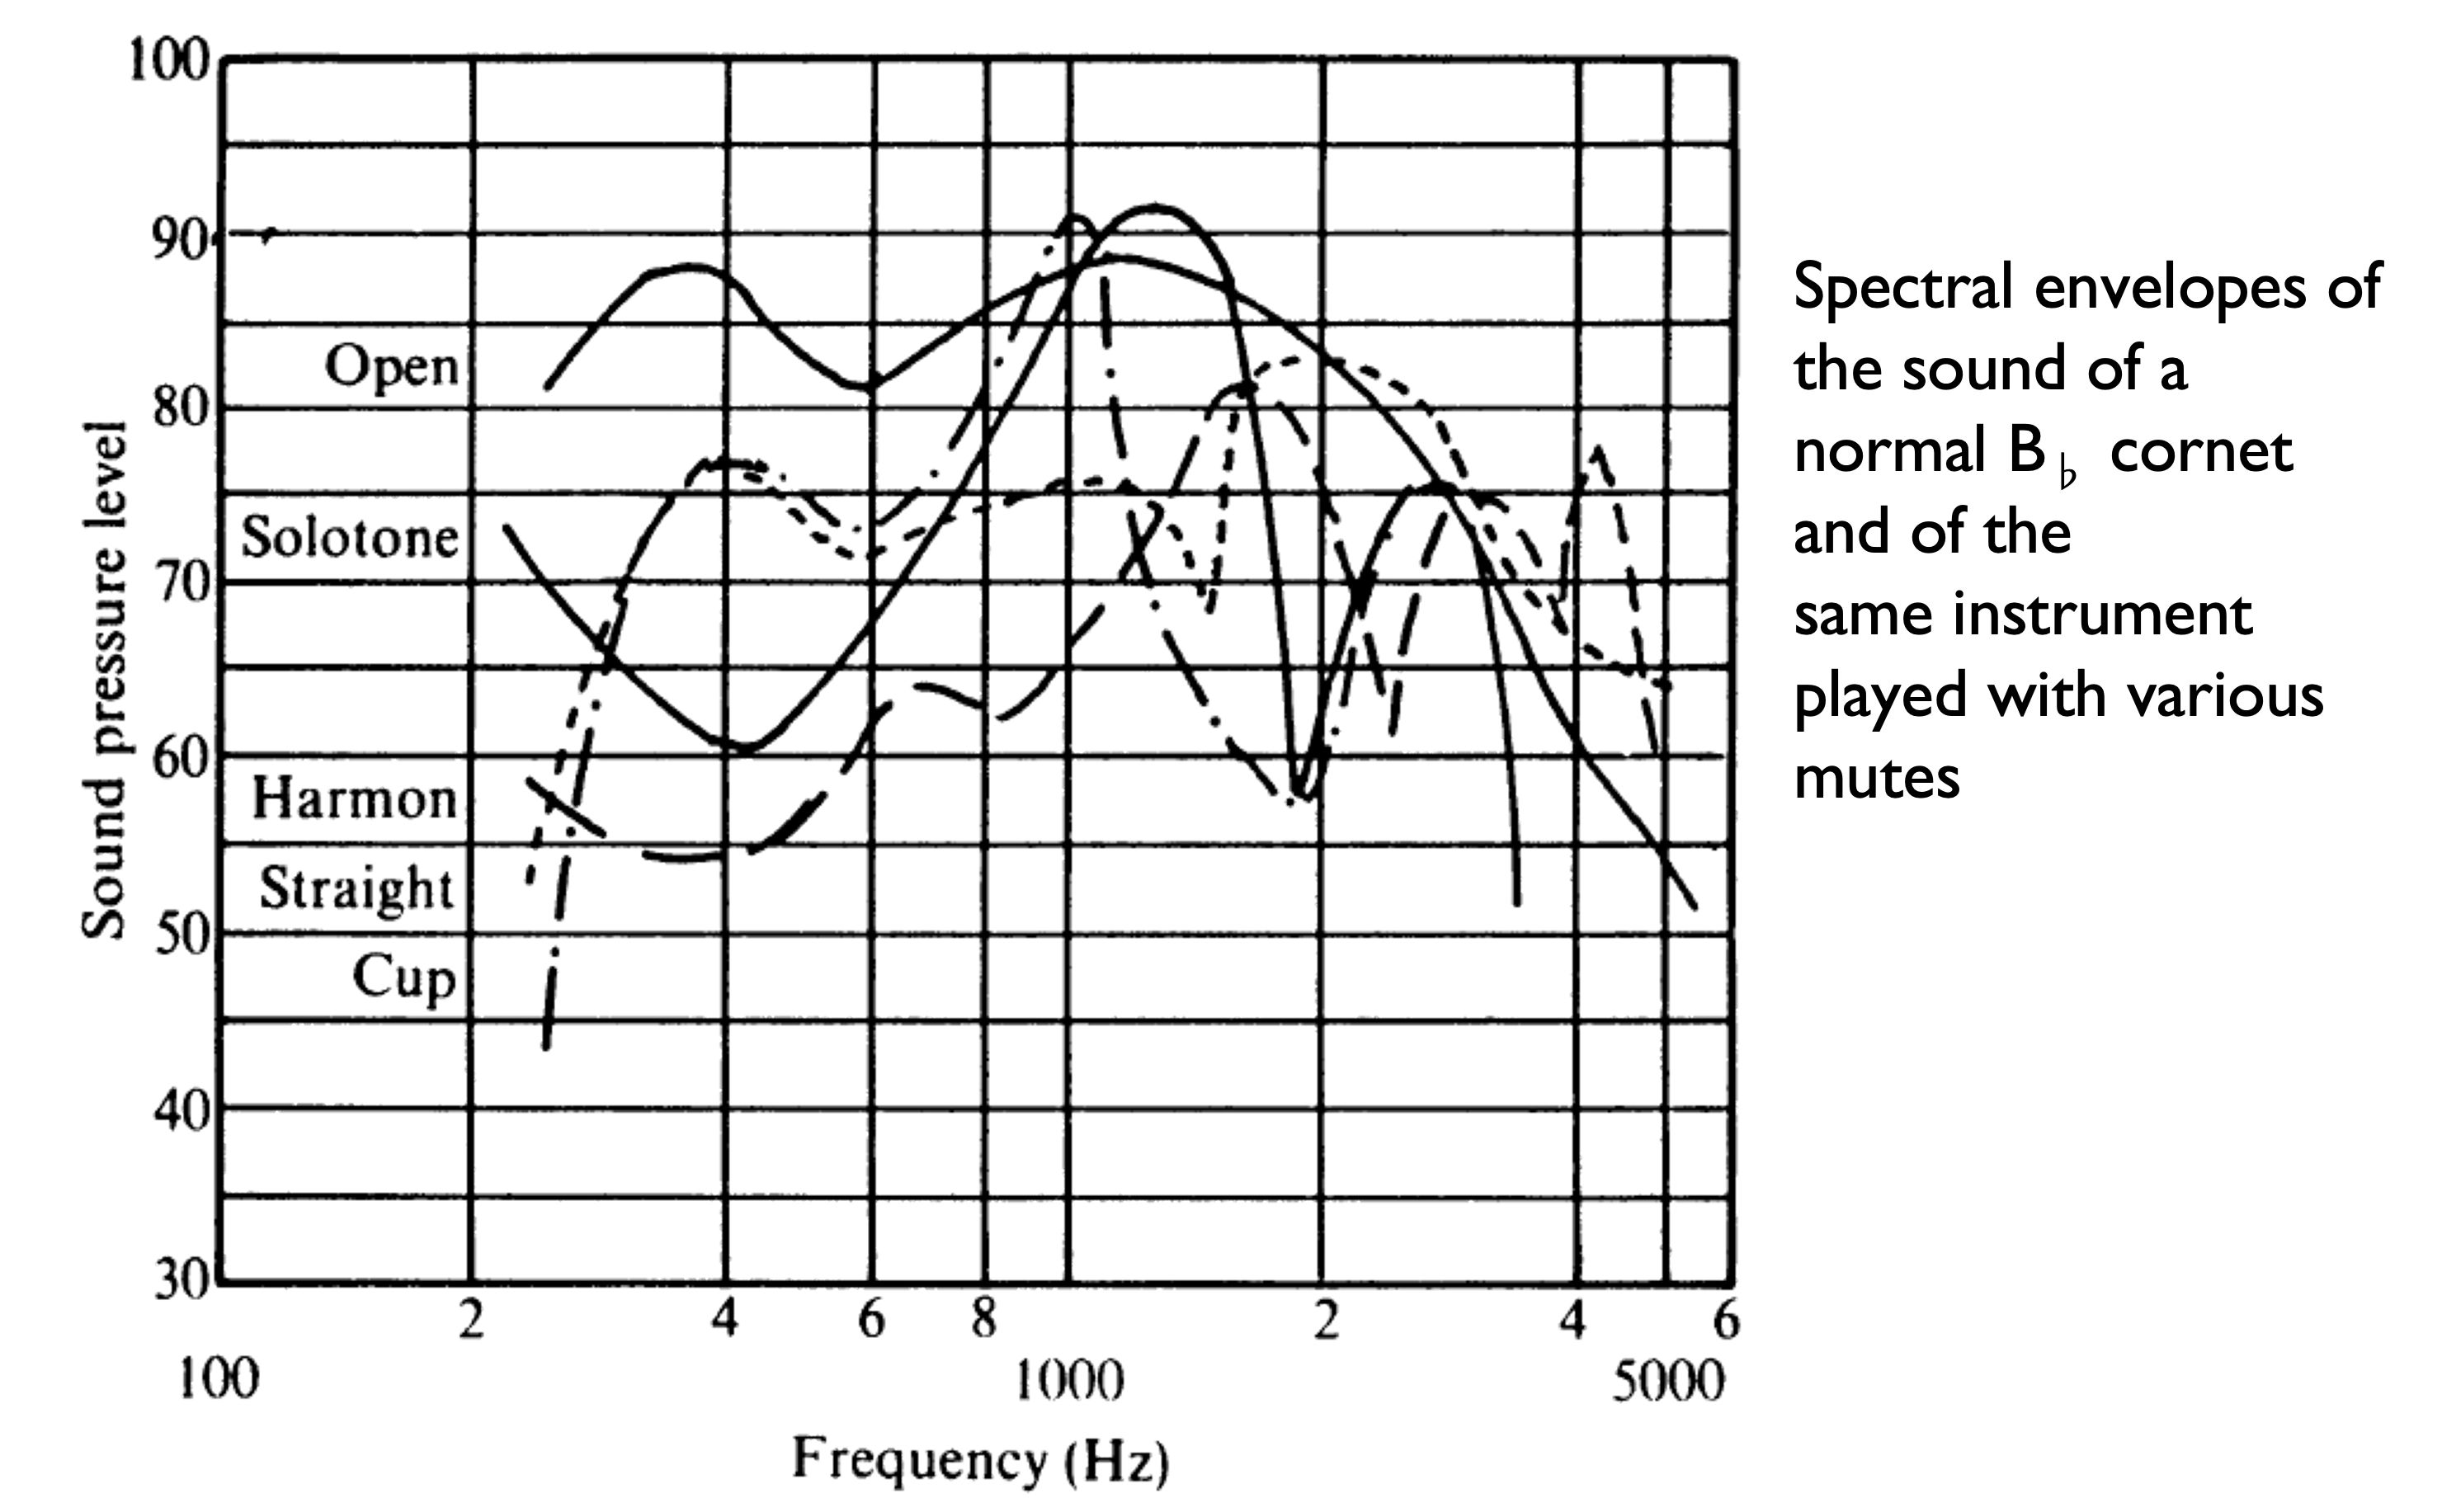
\includegraphics[width=0.7\linewidth]{00_Images/05_chapter/img189.jpg}
\caption{Spectral envelopes with different mutes}
\end{figure}

\paragraph{Considerations} A few recurring acoustic features help to interpret the observed spectral changes.

\begin{itemize}
    \item Most mutes exhibit an admittance maximum, or Helmholtz resonance, associated with their internal cavity, typically in the range \SIrange{200}{300}{\hertz}.
    \item This resonance causes a broad dip in the radiated spectrum around the first and second harmonics over much of the instrument compass, yielding a thinner, reedier, and generally softer sound. 
    \item Additional admittance maxima and minima at higher frequencies are associated with standing waves inside the mute tubes and cavities. 
    \item These higher-frequency resonances and antiresonances lie above about \SI{1000}{\hertz} and contribute strongly to the specific tonal signature of each mute type. 
    \item For some open tube mutes, the radiated sound can be further modified during performance by partially covering the open end with the hand or a cup, producing a wah-wah effect.
\end{itemize}
